% These are the lecture notes for my CSCI360 course SPRING 2017
% at John Jay College of Criminal Justice.

% Feel free to edit these slides and use them for your own courses.
% HOWEVER DO NOT REMOVE THESE LINES!
% Email me at: awood [at] jjay.cuny.edu
% or at: awood [at] gradcenter.cuny.edu


\documentclass{beamer}

\usepackage{tikz}
\usetikzlibrary{calc}

\usepackage{forest}
\usepackage{verbatim}
\usepackage{color}


\setbeamertemplate{footline}[frame number]
\setbeamertemplate{navigation symbols}{} 

\newtheorem{thm}{Theorem}[section]
\newtheorem{lem}{Lemma}
\newtheorem{cl}{Claim}
\newtheorem{cor}{Corollary}[section]
\newtheorem{conj}{Conjecture}
\newtheorem{quest}{Question}
\newtheorem{defn}{Definition}[section]
\newtheorem{obs}{Observation}[section]
\newtheorem{exam}{Example}

\newcommand{\im}{\operatorname{im}}
\newcommand{\id}{\operatorname{id}}
\newcommand{\interior}{\operatorname{int}}
\newcommand{\bdry}{\operatorname{bdry}}
\newcommand{\<}{\langle}
\renewcommand{\>}{\rangle}
\newcommand{\Gab}{(G_\phi)^{ab}} 
\newcommand{\phibar}{\bar{\phi}}
\newcommand{\Z}{\mathbb{Z}}
\newcommand{\N}{\mathbb{N}}
\newcommand{\Q}{\mathbb{Q}}
\newcommand{\R}{\mathbb{R}}
\newcommand{\C}{\mathbb{C}}
\newcommand{\A}{\mathcal{A}}
\newcommand{\OO}{\mathcal{O}}
\newcommand{\UU}{\mathcal{U}}
\newcommand{\power}{2^{\{P_1, \cdots , P_n\}}}
\newcommand{\bp}{\begin{problem}}
\newcommand{\ep}{\end{problem}}
\newcommand{\ba}{\begin{answer}}
\newcommand{\ea}{\end{answer}}
\newcommand{\ds}{\displaystyle}
\newcommand{\ben}{\renewcommand{\theenumi}{\alph{enumi}}
\renewcommand{\labelenumi}{(\theenumi)}\begin{enumerate}}
\newcommand{\een}{\end{enumerate}}
\newcommand{\Hess}{\operatorname{Hessian}}
\newcommand{\Aut}{\mathrm{Aut}}
\newcommand{\Inn}{\mathrm{Inn}}
\newcommand{\Out}{\mathrm{Out}}
\newcommand{\End}{\mathrm{End}}


\mode<presentation>
{
%  \usetheme{default}
  \setbeamercovered{invisible}
}


\usepackage[english]{babel}
\usepackage[latin1]{inputenc}
\usepackage{times}
\usepackage[T1]{fontenc}
\usepackage{stmaryrd}

%\usetheme{default}
%\usetheme{AnnArbor}
%\usetheme{Antibes}
%\usetheme{Bergen}
%\usetheme{Berkeley}
%\usetheme{Berlin}
%\usetheme{Boadilla}
%\usetheme{CambridgeUS}
%\usetheme{Copenhagen}
%\usetheme{Darmstadt}
%\usetheme{Dresden}
%\usetheme{Frankfurt}
%\usetheme{Goettingen}
%\usetheme{Hannover}
%\usetheme{Ilmenau}
%\usetheme{JuanLesPins}
%\usetheme{Luebeck}
%\usetheme{Madrid}
%\usetheme{Malmoe}
%\usetheme{Marburg}
%\usetheme{Montpellier}
%\usetheme{PaloAlto}
%\usetheme{Pittsburgh}
%\usetheme{Rochester}
\usetheme{Singapore}
%\usetheme{Szeged}
%\usetheme{Warsaw}

%\usecolortheme{default}
%\usecolortheme{albatross}
\usecolortheme{beaver}
%\usecolortheme{beetle}
%\usecolortheme{crane}
%\usecolortheme{dolphin}
%\usecolortheme{dove} % grey, white, yellow
%\usecolortheme{fly} %grey, yellow
%\usecolortheme{lily} %white, yellow, blue
%\usecolortheme{orchid}
%\usecolortheme{rose}
%\usecolortheme{seagull}
%\usecolortheme{seahorse}
%\usecolortheme{whale}
%\usecolortheme{wolverine}

% Title page

\title[CSCI360]{Introduction to Modular Arithmetic Using Vigen\`{e}re's Cipher}

\author
{Lecture notes of Alexander Wood \\ CSCI 360 Cryptography and Cryptanalysis \\ \scriptsize \href{mailto:awood@jjay.cuny.edu}{awood@jjay.cuny.edu}}
\institute[JJay]{John Jay College of Criminal Justice}  

\date{}

\begin{document}

% Remove 'figure' text from figure captions 
\setbeamertemplate{caption}{\raggedright\insertcaption\par}

\begin{frame}
  \titlepage
\end{frame}


\begin{frame}
\frametitle{Monoalphabetic Ciphers}

The previous ciphers we have seen, the shift cipher and the substitution cipher, are examples of \textbf{monoalphabetic ciphers} which use a \emph{fixed} substitution over the entire message.
\end{frame}

\begin{frame}
\frametitle{Polyalphabetic Ciphers}

The next big ``leap forward" in cryptography came in the form of \emph{polyalphabetic ciphers}. 
\end{frame}

\begin{frame}
\frametitle{Polyalphabetic Ciphers}

Fun fact: The \textbf{Enigma Machine} from WWII is an example of a (very complex) polyalphabetic cipher.
\end{frame}

\begin{frame}
\frametitle{Vigen\`{e}re's Cipher}

A popular and straightforward polyalphabetic cipher is the \textbf{Vigen\`{e}re Cipher}. Now, a message is encrypted using a predefined \textbf{keyword}.
\end{frame}

\begin{frame}
\frametitle{Intro to Modular Arithmetic}

In order to use Vigen\`{e}re's Cipher we must first learn some basics of \textbf{modular arithmetic}. A common example of modular arithmetic that we are all familiar with is time!
\end{frame}

\begin{frame}
\frametitle{Modular Arithmetic: The Clock}

Consider a clock -- it starts at the top with a $12$. Let's replace this $12$ with a zero. Starting at noon, we are at hour zero and proceed
\[
0, 1, 2, 3, 4, 5, 6, 7, 8, 9, 10, 11, 0, 1, 2, 3, 4, 5, \dots
\]
This is a method of counting \textbf{modulo 12}.
\end{frame}

\begin{frame}
\frametitle{Modulo n}

To count \textbf{modulo 7}, we would count
\[
0, 1, 2, 3, 4, 5, 6, 0, 1, 2, 3, 4, 5, 6, 0, 1, \dots
\]

To count \textbf{modulo n} we count
\[
0, 1, 2, \dots, n-2, n-1, 0, 1, 2, \dots
\]
\end{frame}

\begin{frame}
\frametitle{Residue Classes}

Each integer from $1$ up to $n-1$ can be expressed modulo $n$. We call these the \textbf{residue classes} modulo $n$, sometimes denoted $\mod n$.
\end{frame}

\begin{frame}
\frametitle{Residue Classes}

Any integer can be described as its residue class modulo $n$.

\begin{itemize}
\item $14$ is $4$ modulo $5$, denoted $14 \equiv 4 \pmod 5$.
\item $6$ is $1$ modulo $5$, denoted $6 \equiv 1 \pmod 5$.
\item $17$ is $3$ modulo $14$, denoted $14 \equiv 3 \pmod{17}$. 
\end{itemize}
\end{frame}

\begin{frame}
\frametitle{Residue}

We say that $a$ is the \textbf{modulo-$n$ residue of $b$} when $b \equiv a \pmod n$, and $0\le a < n$.\newline

Note that this residue relates each integer to its remainder after division by the \textbf{modulus} $n$.
\end{frame}




\begin{frame}
\frametitle{Congruence}

\textbf{Congruence} is the mathematical term for equivalence modulo $n$. For instance, $11$ and $1$ are \textbf{congruent} modulo $5$.\newline

In general, $a-b$ are congruent  modulo $n$ if $a-b$ is a multiple of $n$. 
\end{frame}


\begin{frame}
\frametitle{Examples}

\begin{itemize}
\item $31 \equiv 1 \pmod 5$ because $31 - 1 = 30$ is a multiple of $5$.
\item $20 \equiv 13 \equiv 6 \pmod 7$ because $20 - 13 = 7$, $20 - 6 = 14$, and $13 - 6 = 7$.
\item $7 \not\equiv -6 \pmod 3$ because $7 - (-6) = 13$ is not a multiple of $3$.
\end{itemize}
\end{frame}
\begin{frame}
\frametitle{Exercise 1: Residues}

Compute the following residues.

\begin{itemize}
\item $15 \equiv ? \pmod 5$
\item $21 \equiv ?\pmod 5$
\item $4 \equiv ?\pmod 3$
\item $57\equiv ? \pmod{26}$
\end{itemize}
\end{frame}


\begin{frame}
\frametitle{Encoding the Alphabet with Modular Arithmetic} 

We can think of each letter as a number. In this way, $A = 0$, $B = 1$, $C = 2$, et cetera. 
\end{frame}

\begin{frame}
\frametitle{Addition over Encoded Alphabet}

This is useful because we can now add letters as if they were numbers! This provides a quick shortcut from the method we used in our previous codes, where we listed out the letters and performed computations over their indexes. 
\end{frame}

\begin{frame}[fragile]
\frametitle{Addition over Encoded Alphabet}

For example, say we want to encrypt the word \verb|HELLO| by ``adding" the world \verb|LUCKY| to it, ie, by using the \textbf{keyword} \verb|LUCKY|.
\end{frame}


\begin{frame}[fragile]
\frametitle{Addition over Encoded Alphabet}

We would do this letter-by-letter, as before, but using modular arithmetic. We would first compute 
\[
A + L = 7 + 11 = 18 = S
\]
because the letter in the alphabet at index $18$ is S.
\end{frame}

\begin{frame}[fragile]
\frametitle{Addition over Encoded Alphabet}

The last computation we carry out is
\[
O + Y = 14 + 25 = 38
\]
However, there is no index 38 in the alphabet! Thus we must employ computation \textbf{modulo 26}.
\[
38 \equiv 12 \pmod{26}
\]
and hence is encrypted as M.
\end{frame}

\begin{frame}[fragile]
\frametitle{Modular Arithmetic in Python}

The modulus operator in Python is denoted \verb|%|. For instance, $14\pmod 8$ is computed as \verb|14 % 8|, which returns \verb|6|.
\end{frame}


\begin{frame}
\frametitle{Using ASCII}

We can use ASCII as a convenient way of encoding the alphabet. \newline

\url{http://sticksandstones.kstrom.com/appen.html} \newline

However note that instead of having index $0$, instead $A$ has ASCII index $65$ so our encoding will require an extra step. 
\end{frame}

\begin{frame}[fragile]
\frametitle{ASCII in Python}
\begin{itemize}
\item Convert from letters to ASCII in Python using \verb|ord()|:
	\begin{itemize}
	\item \emph{Example:} \verb|ord('A') = 65|
	\end{itemize}
\item Convert from ASCII to letters using \verb|chr()|:
	\begin{itemize}
	\item \emph{Example:} \verb|chr(90) = 'Z'|
	\end{itemize}
\end{itemize}
\end{frame}

\begin{frame}[fragile]
\frametitle{Coding Exercise 1: Encoding The Alphabet with ASCII}

Let's use ASCII and modular arithmetic to write a function, \verb|alph_to_num|, which takes a capital letter as input and converts it to a number between $0$ and $25$ using ASCII codes and modular arithmetic. 
\end{frame}

\begin{frame}[fragile]
\frametitle{Coding Exercise 2: Converting from Numbers Modulo 26 to The Alphabet}

Let's use ASCII and modular arithmetic to write a function, \verb|num_to_alph|, which takes a number modulo $26$ as input and converts it to the corresponding letter in the alphabet using ASCII. 
\end{frame}

\begin{frame}
\frametitle{Vigen\`{e}re's Cipher}

First, Alice (A) and Bob (B) decide upon a keyword. This is done offline, privately. Encryption follows the following steps:
\begin{enumerate}[1)]
\item Write out the plaintext message
\item Below it, write out the keyword, aligning each letter of the keyword below each letter of the plaintext. Repeat the keyword over and over until you reach the end of the plaintext. 
\item ``Add" these letters together using their values modulo 26, as computed in the coding exercises in the previous slides. (\emph{Note that this corresponds to a different Caeser shift for each letter in the keyword!})
\end{enumerate}
\end{frame}

\begin{frame}
\frametitle{A Helpful Chart}

For hand computations we can use the chart provided at \url{http://www.counton.org/explorer/codebreaking/vigenere-cipher.php}. 
\begin{figure}
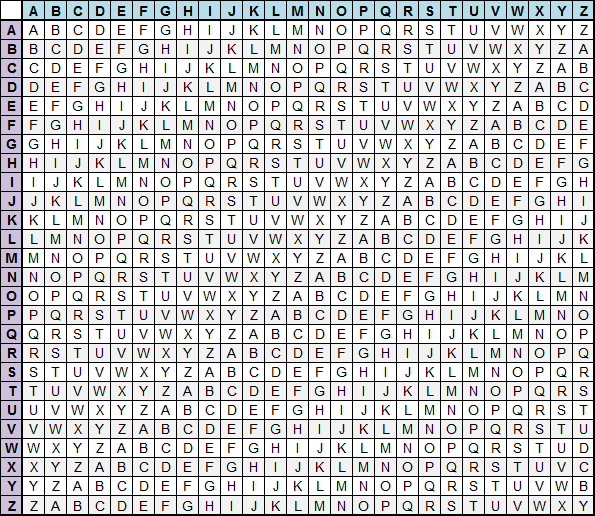
\includegraphics[scale=.4]{IMG/vignere.png}
\end{figure}
\end{frame}

\begin{frame}[fragile]
\frametitle{Execise 2: Viginere's Cipher}
Encrypt the following message by hand using Vigen\`{e}re's cipher. 

\begin{verbatim}
Plaintext:    GOODBYE
Keyword:      LUCKYLU
\end{verbatim}
\end{frame}


\begin{frame}[fragile]
\frametitle{Execise 2: Viginere's Cipher}
Encrypt the following message by hand using Vigen\`{e}re's cipher. 

\begin{verbatim}
Plaintext:    GOODBYE
Keyword:      LUCKYLU
Encryption:   RIQNZJY
\end{verbatim}
\end{frame}

\begin{frame}
\frametitle{Concept Check}

Can we use a straightforward frequency analysis to hack Vigen\`{e}re's cipher, as we could with the substitution cipher? Why or why not? \newline

Brainstorm a new hacking method. (Don't worry about implementing this for now.)
\end{frame}


\begin{frame}
\frametitle{Annoucements}

\begin{itemize}
\item We will have a quiz next class where you will need to:
	\begin{itemize}
	\item Encrypt a short word using Vigen\`{e}re's cipher, given the keyword and the Vigen\`{e}re table.
	\item Perform some basic modular arithmetic. 
	\end{itemize}
\item Remember that Project 1 is due a week from today!
\end{itemize}
\end{frame}

\begin{frame}
\frametitle{References}

\begin{itemize}
\item ASCII chart: \url{http://sticksandstones.kstrom.com/appen.html}
\item Introduction to Modular Arithmetic: 
	\begin{itemize}
	\item \url{https://www.artofproblemsolving.com/wiki/index.php/Modular_arithmetic/Introduction}
	\item \url{https://www.khanacademy.org/computing/computer-science/cryptography/modarithmetic/a/what-is-modular-arithmetic}
	\item A video: \url{https://www.youtube.com/watch?v=Eg6CTCu8iio}
	\end{itemize}
\item Viginere Cipher: \url{http://www.counton.org/explorer/codebreaking/vigenere-cipher.php}
\end{itemize}

\end{frame}
\end{document}


